\chapter{Background}
This chapter explores various works done by the industry as a collective which has allowed for this project to be explored in-depth. 

\section{The Microservice Architecture}
Usually a set of small loosely coupled components that can be deployed, scaled and tested independently making up for a cloud native application, more commonly known as the Microservice architecture.  A major reason for the introduction of this architecture has been the ever increasing demand of deploying cloud native applications as various industries embrace a software driven model. 

Using the microservice architecture comes with it’s own set of unique features, these features allow for new deployment patterns to be discussed and why this paper exists. 

Such features are listed below: 

\begin{itemize}
    \item Highly maintainable and testable 
    \item Loosely coupled with other services 
    \item Independently deployable 
    \item Capable of being deploying by a smaller team
\end{itemize}

\section{Deployment Patterns}
There a few different patterns set out by Chris Richardson, the author of Microservices patterns \cite{Chr19}. These are used to deploy services in different manners to achieve various benefits, i.e cost-effectiveness, speed and scalability. During this dissertation three (only really did 2 in the end) are focused on; 

\subsection{Pattern 1 : Single application per machine}
    \begin{figure}[H]
        \centering
        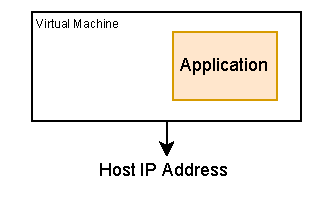
\includegraphics[width=0.5\linewidth]{images/P1_SAPM.pdf}
        \caption{An example application is used for visualizing the pattern mentioned here.}
    \end{figure}  

A basic pattern in which a single microservice application is deployed on one machine, this allows for a simple and cost effective deployment depending on the use-case scenario. The ideal scenario would fit an application with a small user-base however would see themselves grow within the future to utilize the various advantages of the microservice architecture. 

\subsection{Pattern 2 : }

\section{Azure}

